% lecture04.tex: Lecture 4: Chemical Differentiation & Magnetospheres
% Planetary Systems, Kapteyn Institute

\documentclass[aspectratio=169, 11pt]{beamer}

% ── Theme and macros ────────────────────────────────────────
\usepackage{../common/beamerthemeIPS}
% macros.tex: Shared math macros for IPS lecture slides
% Mirrors definitions in book/_config.yml for consistency
% Uses \providecommand to avoid conflicts with unicode-math

% ── Derivatives ─────────────────────────────────────────────
\providecommand{\dv}[2]{\frac{\mathrm{d} #1}{\mathrm{d} #2}}
\providecommand{\dd}{}\renewcommand{\dd}{\mathrm{d}}
\providecommand{\pdv}[2]{\frac{\partial #1}{\partial #2}}

% ── Solar quantities ────────────────────────────────────────
\newcommand{\Msun}{M_{\odot}}
\newcommand{\Rsun}{R_{\odot}}
\newcommand{\Lsun}{L_{\odot}}

% ── Planetary quantities ────────────────────────────────────
\newcommand{\Mearth}{M_{\oplus}}
\newcommand{\Rearth}{R_{\oplus}}
\newcommand{\Mjup}{M_{\mathrm{J}}}
\newcommand{\Rjup}{R_{\mathrm{J}}}

% ── Constants ───────────────────────────────────────────────
\newcommand{\kB}{k_{\mathrm{B}}}

% ── Media links ─────────────────────────────────────────────
% Clickable button that opens the animated or video version of a
% figure, e.g. \mediabutton{https://...gif}{Play animation}
\providecommand{\mediabutton}[2]{\href{#1}{\beamergotobutton{#2}}}

\graphicspath{{figures/}{../common/}{../../book/04_differentiation_magnetospheres/figures/}}

% ── Metadata ────────────────────────────────────────────────
\title[Lecture 4: Differentiation \& Magnetospheres]{Lecture 4: Chemical Differentiation\\\& Magnetospheres}
\subtitle{Planetary Systems}
\author[L4]{Tim Lichtenberg}
\institute{Kapteyn Astronomical Institute\\University of Groningen}
\date{2026}
\titlebgcredit{Aurora australis, ISS. Credit: NASA}

% ════════════════════════════════════════════════════════════
\begin{document}

% ── Title slide ─────────────────────────────────────────────
\begin{frame}[plain,noframenumbering]
  \titlepage
\end{frame}

% ── Learning objectives ─────────────────────────────────────
\begin{frame}{Learning objectives}
  By the end of this lecture, you will be able to:
  \vskip8pt
  \begin{itemize}
    \item Explain metal--silicate separation and core formation
    \item Use siderophile element depletion as evidence for differentiation
    \item Describe the Hf--W chronometer for dating core formation
    \item Derive the magnetic Reynolds number and assess dynamo feasibility
    \item Compare magnetic fields across the solar system
  \end{itemize}
\end{frame}

% ── Recap ───────────────────────────────────────────────────
\begin{frame}{Recap: Lecture 3}
  \begin{itemize}
    \item Four heat sources: accretional, differentiation, radioactive, tidal
    \item Conduction too slow for planets: $\tau \sim L^2/\kappa$
    \item Rayleigh number: $\mathrm{Ra} \sim 10^7$--$10^8$ for Earth $\Rightarrow$ vigorous convection
    \item Plate tectonics (mobile lid) vs.\ stagnant lid
    \item Tidal heating: Io, Enceladus, Europa
  \end{itemize}
  \vskip8pt
  \textbf{Today:} The \textit{chemical} consequences of melting, and how differentiation enables magnetic fields.
\end{frame}

% ════════════════════════════════════════════════════════════
\sectionimage{planetary_differentiation}{Planetary differentiation. Credit: Wikimedia, CC BY-SA 4.0}
\section{Accretion, melting, \& core formation}
% ════════════════════════════════════════════════════════════

% ── Metal-silicate separation ──────────────────────────────
\begin{frame}{Metal--silicate separation}
  \begin{columns}[c]
    \column{\recapfigcolnarrow}
    \centering
    \ipsrecapfig{planetary_differentiation}
    \source{Wikimedia, CC BY-SA 4.0}

    \column{\recaptextcolwide}
    \begin{itemize}
      \item Accretional heating + ${}^{26}\mathrm{Al}$ $\rightarrow$ \textbf{magma ocean}
      \item Iron ($\rho \sim 7000$~kg\,m$^{-3}$) is immiscible with silicate ($\rho \sim 3000$~kg\,m$^{-3}$)
      \item Iron droplets sink through silicate melt
      \item \textbf{Stokes settling velocity:}
      $$v_{\mathrm{Stokes}} = \frac{2}{9}\frac{\Delta\rho\,g\,r^2}{\mu}$$
      \item cm droplets: $v \sim 4$~m\,s$^{-1}$ (Stokes), $\sim$0.5~m\,s$^{-1}$ with turbulent drag
    \end{itemize}
  \end{columns}
\end{frame}

\begin{frame}
  \centering
  \makebox[\linewidth][c]{\includegraphics[width=0.95\paperwidth, height=0.64\paperheight, keepaspectratio]{stokes_settling}}\\
  {\footnotesize Stokes settling of iron droplets in a magma ocean: $v \propto r^2$ (slope 2 on log-log axes), 0.044 m\,s$^{-1}$ at 1 mm and 4.4 m\,s$^{-1}$ at 1 cm. Left of the dashed line ($\mathrm{Re} \approx 1$) Stokes' law holds; to its right the flow is turbulent and a 1 cm droplet moves nearer 0.5 m\,s$^{-1}$, still crossing a 1000 km magma ocean within weeks. Iron rain empties a magma ocean of its metal within weeks: on geological clocks, core formation is instantaneous. Course figure.}
\end{frame}

\begin{frame}{The magma ocean state, and why it is essential}
  After accretion the outer few thousand kilometres of a terrestrial planet are molten: depth several hundred to $>$2000 km, surface temperature 2000--4000 K, viscosity $10^{-1}$--$10^{0}$ Pa\,s, turbulent convection ($\mathrm{Ra} \gtrsim 10^{25}$), cooling set by surface radiation and greenhouse blanketing.
  \vskip6pt
  \begin{itemize}\setlength\itemsep{2pt}
    \item \textbf{Liquid mantle:} iron droplets sink at m\,s$^{-1}$, a core forms within weeks
    \item \textbf{Solid mantle:} rock flows so slowly ($\mu \sim 10^{21}$ Pa\,s, 22 orders of magnitude above silicate melt) that even a km-sized iron body would need longer than the age of the universe to reach the centre
    \item Magma ocean lifetime $10^3$--$10^8$ yr: long enough for core formation, short compared to planetary evolution
  \end{itemize}
  \vskip6pt
  \keyresult{Core formation happens while the planet is molten, or not at all; chondritic asteroids that never melted never formed cores.}
\end{frame}

% ── Magma ocean state ──────────────────────────────────────

% ── Moon-forming impact ────────────────────────────────────
\begin{frame}{The Moon-forming giant impact}
  \begin{itemize}
    \item Mars-sized body (Theia) collided with proto-Earth $\sim$4.5~Ga
    \item Re-melted most of Earth's mantle, vaporised part of it
    \item Created the final deep magma ocean
    \item Established present core--mantle structure
    \item Debris disk $\rightarrow$ Moon (confirmed by lunar $\varepsilon^{182}\mathrm{W}$ matching Earth's mantle)
  \end{itemize}
  \vskip8pt
  \keyresult{Core formation is not a single event but a series of episodes, culminating in the giant impact.}
\end{frame}

\begin{frame}
  \centering
  \makebox[\linewidth][c]{\includegraphics[width=0.95\paperwidth, height=0.70\paperheight, keepaspectratio]{kegerreis2022_moon_impact}}\\
  {\footnotesize SPH simulation of the Moon-forming giant impact: (a) Mars-sized Theia approaches the proto-Earth, (b) contact and tidal disruption, (c) part of the debris falls back while outer clumps survive, (d) a satellite on a wide orbit. Kegerreis et al.\ (2022).}\\[2pt]
  \mediabutton{https://ips.formingworlds.space/_images/kegerreis2022_moon_impact.gif}{Play animation}\hspace{6pt}\mediabutton{https://www.youtube.com/watch?v=gFYZ9k0aFsk}{Source video}
\end{frame}

\begin{frame}{Giant impacts that remove mantles}
  Not every giant impact ends in net accretion: an oblique, fast collision can strip more silicate than it delivers.
  \vskip6pt
  \begin{itemize}
    \item \textbf{Mercury:} core mass fraction $\sim$74\% (Earth $\sim$32\%, Mars $\sim$24\%); a hit-and-run impact (an oblique collision whose remnant re-accretes rather than merging) stripped $\sim$50--70\% of the pre-impact mantle
    \item \textbf{Mars:} the hemispheric dichotomy ($\sim$6 km elevation, $\sim$30 km crustal-thickness contrast) is the relaxed scar of a Borealis-scale impact; crust moved sideways, not lost
    \item \textbf{Earth--Moon:} the opposite endpoint, net accretion of the impactor
  \end{itemize}
  \vskip6pt
  \keyresult{Mercury and Earth are the two endpoints of the same process: giant impacts set the final core-to-mantle ratio.}
  \vskip4pt
  \sourcenote{Benz et al.\ (2007); Chau et al.\ (2018); Andrews-Hanna et al.\ (2008); Marinova et al.\ (2008)}
\end{frame}

\begin{frame}
  \centering
  \makebox[\linewidth][c]{\includegraphics[width=0.95\paperwidth, height=0.64\paperheight, keepaspectratio]{chau2018_mercury_impact}}\\
  {\footnotesize A mantle-stripping giant impact on proto-Mercury (SPH simulation): a proto-Mercury of 2.25 present Mercury masses (red core, yellow mantle) is hit by an impactor of half its mass at impact parameter $b = 0.5$ and $v = 30$ km\,s$^{-1}$; the white bar marks $1\,\Rearth$. Silicate is ejected while the metal-rich remnant recollapses; after 53 hours the largest fragment holds 0.95 Mercury masses with iron mass fraction $Z_\mathrm{Fe} = 0.67$. One oblique collision at several escape velocities converts an ordinary protoplanet into iron-rich Mercury. Chau et al.\ (2018).}
\end{frame}

\begin{frame}
  \centering
  \makebox[\linewidth][c]{\includegraphics[width=0.95\paperwidth, height=0.74\paperheight, keepaspectratio]{mola_mars_topography}}\\
  {\footnotesize Mars's hemispheric dichotomy in MOLA global topography: smooth, low northern plains (blue) against cratered southern highlands (orange to red); the deep blue basin on the right is Hellas. Credit: NASA/JPL.}
\end{frame}

% ── Late veneer ────────────────────────────────────────────
\begin{frame}{The late veneer}
  Highly siderophile elements (Ir, Pt, Os, Au) are \textbf{overabundant} in Earth's mantle compared to the deep-core equilibration prediction.
  \vskip6pt
  \begin{itemize}
    \item Mantle abundances $\sim$200$\times$ higher than expected for full metal extraction
    \item Relative ratios are \textbf{chondritic} (matching primitive meteorites), not fractionated
    \item Interpretation: an extra $\sim$0.5\% of Earth's mass accreted \textbf{after} core formation closed
    \item This ``late veneer'' delivered its siderophile elements to the mantle without equilibrating with the core
  \end{itemize}
  \vskip6pt
  \sourcenote{Walker (2009); Day et al.\ (2016)}
  \vskip4pt
  \flushleft
  A smaller late veneer is also inferred for Mars and the Moon from their platinum-group element abundances.
\end{frame}

% ── Goldschmidt classification ─────────────────────────────
\begin{frame}{Goldschmidt classification}
  \begin{columns}[c]
    \column{\recapfigcolnarrow}
    \centering
    \ipsrecapfig{goldschmidt_classification}
    \source{Wikimedia, CC BY-SA 3.0}

    \column{\recaptextcolwide}
    \footnotesize
    \setlength\tabcolsep{4pt}
    \begin{tabular}{@{}l l l@{}}
      \toprule
      \textbf{Class} & \textbf{Affinity} & \textbf{Examples} \\
      \midrule
      Siderophile & Core (metal) & Fe, Ni, Pt, Au \\
      Lithophile & Mantle (silicate) & Si, Mg, Al, U, Th \\
      Chalcophile & Sulfide & Cu, Zn, Pb \\
      Atmophile & Gas & H, C, N, noble \\
      \bottomrule
    \end{tabular}
    \vskip6pt
    The depletion of siderophile elements in Earth's mantle is \textbf{direct evidence} for core formation.
  \end{columns}
\end{frame}

% ── Partition coefficients ────────────────────────────────
\begin{frame}{Partition coefficients, and why silicon is in the core}
  \begin{columns}[c]
    \column{0.48\textwidth}
    \centering
    $D_i^{\mathrm{met/sil}} \equiv C_i^{\mathrm{metal}} / C_i^{\mathrm{silicate}}$
    \vskip4pt
    \footnotesize
    \setlength\tabcolsep{3pt}
    \begin{tabular}{l c l}
      \toprule
      \textbf{Element} & $\boldsymbol{D^{\mathrm{met/sil}}}$ & \textbf{Behaviour} \\
      \midrule
      Ir, Os, Pt & $10^4$--$10^6$ & Highly siderophile \\
      W, Mo      & $10^2$--$10^4$ & Moderately siderophile \\
      Ni, Co     & 10--100        & Weakly siderophile \\
      Fe         & $\sim$10        & Weakly siderophile \\
      Si, Mg, O  & $\ll 1$         & Lithophile \\
      \bottomrule
    \end{tabular}
    \column{0.50\textwidth}
    \small
    $D$ depends on pressure, temperature and oxygen fugacity (an effective O$_2$ partial pressure that sets the redox state of the melt):
    \begin{itemize}\setlength\itemsep{2pt}
      \item Earth's mantle is depleted $\sim$1000$\times$ in Ir and Pt: the iron-loving elements followed the metal into the core
      \item Si is lithophile below 10 GPa, but $D_\mathrm{Si}$ rises to $\sim$1 at 40--60 GPa: the core holds several wt\% Si, part of its 5--10\% density deficit (Lecture 8)
    \end{itemize}
  \end{columns}
  \keyresult{Deep magma ocean partitioning at 40--60 GPa is the standard model for Earth's core composition.}
  \sourcenote{Rubie et al.\ (2015); Fischer et al.\ (2015); Hirose et al.\ (2021); Shahar et al.\ (2026)}
\end{frame}

% ── Partition coefficient pressure dependence ────────────

\begin{frame}
  \centering
  \makebox[\linewidth][c]{\includegraphics[width=0.95\paperwidth, height=0.56\paperheight, keepaspectratio]{siebert2013_partition_coefficients}}\\
  {\footnotesize Metal-silicate partition coefficients against pressure: laboratory $D^{\mathrm{met/sil}}$ for Ni and Co at magma-ocean conditions. At low pressure $D \sim 10^3$--$10^4$, so the mantle should keep almost no Ni or Co; the grey band ($D \approx 24$--26) is the value required by the Ni and Co the mantle actually holds. Both curves reach the band only near 40--60 GPa: equilibration at $54 \pm 5$ GPa, the base of a 1000--1500 km deep magma ocean (Fischer et al.\ 2015). The mantle's siderophile depletions remember the depth at which the core formed. Course figure, after Siebert et al.\ (2013).}
\end{frame}

% ── Hf-W chronometry ──────────────────────────────────────
\begin{frame}{Hf--W chronometry: when did cores form?}
  ${}^{182}\mathrm{Hf} \rightarrow {}^{182}\mathrm{W}$, half-life 8.9 Myr. Hf is lithophile (stays in the mantle), W is siderophile (goes to the core). Early core formation strips W while ${}^{182}\mathrm{Hf}$ is still alive, so the mantle builds an excess of ${}^{182}\mathrm{W}$; late core formation (after ${}^{182}\mathrm{Hf}$ is gone) leaves the mantle chondritic, $\varepsilon^{182}\mathrm{W} \approx 0$.
  \vskip6pt
  \centering
  \small
  \begin{tabular}{l l l}
    \toprule
    \textbf{Body} & $\boldsymbol{\varepsilon^{182}\mathrm{W}}$ & \textbf{Core formation timing} \\
    \midrule
    Earth & $+2$ & two-stage age $\sim$30 Myr, a lower limit \\
    Mars  & $+0.4$ bulk, $+1.8$ shergottites & complete within $\sim$10 Myr \\
    Moon  & $\sim$Earth & consistent with the giant impact \\
    \bottomrule
  \end{tabular}
  \vskip4pt
  \flushleft
  \small Earth's bulk core formation finished within $\sim$100 Myr; depleted shergottites are a martian meteorite class.
  \vskip2pt
  \sourcenote{Kleine et al.\ (2009); Nimmo \& Kleine (2015); Kleine \& Walker (2017)}
\end{frame}

% ── Hf-W evolution schematic ──────────────────────────────

\begin{frame}
  \centering
  \makebox[\linewidth][c]{\includegraphics[width=0.95\paperwidth, height=0.72\paperheight, keepaspectratio]{hf_w_schematic}}\\
  {\footnotesize (a) Core formation separates parent (Hf, mantle) from daughter reservoir (W, core). (b) Mantle $^{182}$W excess vs.\ time of core formation, two-stage model with Earth's mantle Hf/W: the measured $+2\,\varepsilon$ gives $\sim$28 Myr. Course figure.}
\end{frame}

\begin{frame}
  \centering
  \makebox[\linewidth][c]{\includegraphics[width=0.95\paperwidth, height=0.55\paperheight, keepaspectratio]{accretion_core_formation_timeline}}\\
  {\footnotesize (a) The first 5 Myr after CAI condensation (CAIs, calcium-aluminium-rich inclusions, the first nebular solids, define $t = 0$): chondrules and planetesimals within $\sim$4 Myr (Lecture 12). (b) Core formation to 300 Myr: planetesimal cores (iron meteorites) by $\sim$1--3 Myr, Mars within $\sim$10 Myr, Earth's two-stage age of $\sim$30 Myr as a lower limit with completion within $\sim$100 Myr, the Moon-forming impact after $\sim$50 Myr. Small bodies differentiate within 1--3 Myr; Earth needs tens of Myr. Course figure, after Lichtenberg et al.\ (2023); ages from Nimmo \& Kleine (2015), Kleine \& Walker (2017), Kruijer et al.\ (2017).}
\end{frame}

% ── Mantle differentiation ─────────────────────────────────

\begin{frame}
  \centering
  \makebox[\linewidth][c]{\includegraphics[width=0.95\paperwidth, height=0.55\paperheight, keepaspectratio]{magma_ocean_adiabats}}\\
  {\footnotesize Peridotite solidus and liquidus against magma-ocean adiabats at successive times $t_1$--$t_4$. The melting curves rise more steeply with pressure than the adiabats, so the cooling adiabat first meets the liquidus at the base ($t_2$, open circle), where bridgmanite (MgSiO$_3$) crystallises first; the adiabat-solidus intersection (dots) is the crystallisation front, shallower at each later time; between the curves crystals and melt coexist as mush. Caveat: dense Fe-rich melt can survive at the base as a basal magma ocean (Labrosse et al.\ 2007; Samuel et al.\ 2023). Deep magma oceans crystallise from the bottom up. Course figure, after Elkins-Tanton (2012).}
\end{frame}

% ── Incompatible element enrichment ──────────────────────
\begin{frame}{Incompatible elements and mantle reservoirs}
  Large ions (U$^{4+}$, Th$^{4+}$, K$^+$) fit poorly into crystal lattices, concentrate in the shrinking residual liquid and end up in the crust: continental crust is 50--100$\times$ enriched in U, Th and K over the upper mantle, and about half of Earth's radiogenic heat comes from a crust that is $<$1\% of its mass.
  \vskip4pt
  \begin{description}
    \item[DMM] \textbf{Depleted MORB Mantle}: upper-mantle source of mid-ocean ridge basalts, depleted by partial melting and crustal extraction.
    \item[EM/OIB] \textbf{Enriched Mantle}: deep plumes sample primordial mantle or recycled oceanic crust with preserved incompatible elements.
    \item[HIMU] ``High-$\mu$'' reservoir: high U/Pb, likely very old subducted oceanic crust.
  \end{description}
  \vskip2pt
  \keyresult{Isotopic diversity of ocean island basalts (Hawaii, Iceland, Samoa) is direct evidence for long-lived mantle heterogeneity.}
\end{frame}

\begin{frame}
  \centering
  \makebox[\linewidth][c]{\includegraphics[width=0.95\paperwidth, height=0.64\paperheight, keepaspectratio]{mantle_reservoirs}}\\
  {\footnotesize Mantle reservoirs after magma ocean crystallisation and later melting. The depleted MORB mantle, source of mid-ocean ridge basalts, lost its incompatible elements to the continental crust. The enriched mantle sampled by plumes, source of ocean island basalts, holds primordial material or recycled oceanic crust. Course schematic.}
\end{frame}

% ── Mantle reservoirs ─────────────────────────────────────

% ── Lunar magma ocean ─────────────────────────────────────
\begin{frame}{The lunar magma ocean: direct evidence}
  The Moon shows the clearest record of magma ocean differentiation:
  \vskip4pt
  \begin{itemize}
    \item The concept was born from Apollo 11: anorthosite fragments in the Mare Tranquillitatis soil led Wood et al.\ (1970) to propose a deep molten shell
    \item \textbf{Anorthositic highlands:} low-density plagioclase feldspar floated to the top of the crystallising lunar magma ocean $\sim$4.4~Ga
    \item Apollo samples of anorthosite date to 4.36--4.44~Ga (within 200~Myr of solar system formation)
    \item \textbf{KREEP} layer: the last dregs of crystallisation, rich in \textbf{K}, \textbf{R}are \textbf{E}arth \textbf{E}lements, \textbf{P}hosphorus; shallow under the nearside maria
    \item Lunar crust thickness varies from $\sim$30~km (nearside) to $\sim$70~km (farside)
  \end{itemize}
  \vskip4pt
  \keyresult{The Moon is the textbook case of magma ocean differentiation; its exposed anorthosite confirms the theoretical crystallisation sequence.}
\end{frame}

\begin{frame}
  \centering
  \makebox[\linewidth][c]{\includegraphics[width=0.95\paperwidth, height=0.56\paperheight, keepaspectratio]{lunar_magma_ocean_cutout}}\\
  {\footnotesize End-state of the lunar magma ocean (thin layers exaggerated): the 40--50 km anorthosite flotation crust, beneath it the yellow urKREEP layer, the last $\sim$1\% of liquid to solidify; light green pyroxenite and dunite cumulates; the dark green ilmenite-rich cumulates formed late in the sequence and are denser than everything below, so they sink (mantle overturn) in the first $\sim$500 Myr; an iron core at the centre. Apollo samples match this stratigraphy in detail: the Moon is the clearest test case of magma-ocean theory. Course figure, after Elkins-Tanton (2012).}
\end{frame}

\begin{frame}
  \centering
  \makebox[\linewidth][c]{\includegraphics[width=0.95\paperwidth, height=0.80\paperheight, keepaspectratio]{moon_nearside_annotated}}\\
  {\footnotesize The bright highlands are the anorthositic flotation crust; the dark maria are later lava flows. Credit: NASA/GSFC/Arizona State University (LROC WAC mosaic), public domain.}
\end{frame}

% ── Volatile delivery: classical vs modern ────────────────

\begin{frame}
  \centering
  \makebox[\linewidth][c]{\includegraphics[width=0.95\paperwidth, height=0.45\paperheight, keepaspectratio]{volatile_delivery_schematic}}\\
  {\footnotesize Classical versus revised picture of volatile delivery. (a) Classical: a fixed snow line keeps the inner disk dry, and water arrives late by asteroids and comets scattered inward. (b) Revised: the snow line (the radius beyond which water condenses as ice) sweeps outward, then retreats; the earliest inner planetesimals form beyond it and accrete ice (blue bodies), and Jupiter's growth blocks the inward pebble drift and splits the disk into the NC and CC reservoirs. The protoplanets then dry out again by ${}^{26}$Al melting, impact devolatilisation and pebble ablation in primordial atmospheres; most of Earth's remaining water was present at accretion, not delivered afterwards. Course figure, after Alexander et al.\ (2019), Lichtenberg et al.\ (2021), Grewal et al.\ (2024).}
\end{frame}

% ── Outgassing from the magma ocean ───────────────────────
\begin{frame}{Outgassing and volatile solubility}
  \small
  As the magma ocean cools, dissolved volatiles outgas; speciation follows the \textbf{oxygen fugacity} $f_{\mathrm{O}_2}$ of the mantle: reducing (low $f_{\mathrm{O}_2}$) gives H$_2$, CO, N$_2$, CH$_4$; oxidising (high $f_{\mathrm{O}_2}$) gives H$_2$O, CO$_2$, N$_2$, SO$_2$.
  \vskip4pt
  Each gas dissolves through its own reaction with the melt: H$_2$O as hydroxyl groups, CO$_2$ as carbonate ions ($\sim$100$\times$ less soluble), N as nitrides only when reduced, S as sulfide or sulfate. Each water molecule splits into two OH groups:
  \keyresult{$$X_{\mathrm{H_2O}} \propto p_{\mathrm{H_2O}}^{1/2}$$}
  A thicker steam atmosphere lets the magma retain more water: a self-limiting feedback, so a planet cannot outgas its entire water budget. The mantle redox state at solidification sets the initial atmosphere (Lectures 5--6).
  \sourcenote{Hirschmann (2012)}
\end{frame}

% ── Volatile solubility in silicate melt ──────────────────

\begin{frame}
  \centering
  \makebox[\linewidth][c]{\includegraphics[width=0.95\paperwidth, height=0.55\paperheight, keepaspectratio]{outgassing_speciation_fO2}}\\
  {\footnotesize Volatile partitioning between magma ocean and atmosphere against oxygen fugacity (equilibrium outgassing model of Nicholls et al.\ 2024, bulk silicate Earth inventory of Krijt et al.\ 2023). (a) The melt keeps almost the whole water inventory dissolved ($\sim 5 \times 10^{21}$ kg, over 3 present-day oceans) at all but the most reducing conditions. (b) Carbon is far less soluble: CO$_2$ and CO fill the atmosphere at hundreds to thousands of bar while steam stays at a few bar; H$_2$, CO and CH$_4$ when reduced, CO$_2$ then SO$_2$ when oxidised. During the magma ocean stage most of the water sits in the magma, not in the atmosphere.}
\end{frame}

\begin{frame}{Impact erosion and delivery}
  \small
  \begin{itemize}\setlength\itemsep{2pt}
    \item \textbf{Local:} an ordinary impactor removes at most the air above the tangent plane, a fraction $H/2R \approx 6 \times 10^{-4}$ of Earth's atmosphere per event; erosion is cumulative, and km-scale planetesimals erode most efficiently per unit mass
    \item \textbf{Global:} a giant impact shakes the whole planet and air is lost wherever the ground approaches $v_\mathrm{esc}$; even the Moon-forming impact removes only $\sim$20\%, more with a surface ocean
    \item The same planetesimals also deliver volatiles; Venus keeps $\sim$50$\times$ more $^{36}\mathrm{Ar}$ than Earth because oceans on proto-Earth enhanced its loss
    \item A primordial H$_2$-He envelope dies by attrition: repeated impacts plus XUV-driven thermal escape (Lecture 5)
  \end{itemize}
  \vskip2pt
  \keyresult{Earth's air and oceans are the ledger of delivery minus erosion, closed by magma-ocean outgassing.}
  \sourcenote{Melosh \& Vickery (1989); Genda \& Abe (2003, 2005); Schlichting et al.\ (2015)}
\end{frame}

\begin{frame}
  \centering
  \makebox[\linewidth][c]{\includegraphics[width=0.95\paperwidth, height=0.74\paperheight, keepaspectratio]{roche2025_impact_loss}}\\
  {\footnotesize Atmospheric loss in a giant impact: ejecta plumes drive near-field loss at the impact site, while the shock breaking out on the far side drives far-field loss; green particles are lost. Roche et al.\ (2025), CC BY 4.0.}
\end{frame}

% ── NC-CC dichotomy ───────────────────────────────────────
\begin{frame}{Meteoritic dichotomy: NC vs.\ CC}
  Meteorites split into two isotopic groups: \textbf{non-carbonaceous (NC)} and \textbf{carbonaceous (CC)}.
  \vskip6pt
  \begin{itemize}
    \item NC and CC have distinct $^{50}\mathrm{Ti}$, $^{54}\mathrm{Cr}$, $^{48}\mathrm{Ca}$ ratios
    \item They reflect two separate reservoirs in the early solar nebula
    \item Interpretation: \textbf{Jupiter} formed early, blocking mixing between inner and outer disk
    \item Both reservoirs contributed to Earth's accretion, but in changing proportions over time
  \end{itemize}
  \vskip6pt
  \sourcenote{Kruijer et al.\ (2017); Lichtenberg et al.\ (2021)}
  \vskip4pt
  \flushleft
  This dichotomy is one of the strongest meteoritic constraints on the timing of giant planet formation.
\end{frame}

% ════════════════════════════════════════════════════════════
\sectionimage{geodynamo_schematic}{Geodynamo. Credit: Wikimedia, CC BY-SA 4.0}
\section{Planetary dynamos}
% ════════════════════════════════════════════════════════════

% ── Space weather consequences ───────────────────────────
\begin{frame}{Why magnetic fields matter}
  \begin{itemize}\setlength\itemsep{3pt}
    \item \textbf{Atmospheric shielding:} deflects the solar wind and reduces ion sputtering (atoms knocked loose by particle impacts) of the upper atmosphere; Mars lost its field $\sim$4 Ga and then $\sim$0.8 bar of atmosphere (MAVEN)
    \item \textbf{Surface habitability:} limits the cosmic-ray flux and radiation dose at the surface, protects the ozone layer from charged particles; on Venus the missing field is one likely contributor to hydrogen escape
    \item \textbf{Geological record:} magnetic minerals record the field history (paleomagnetism)
    \item \textbf{Interior probe:} field properties constrain the deep interior
    \item Debated: how essential is a global field for a habitable surface?
  \end{itemize}
  \vskip4pt
  \sourcenote{Lammer et al.\ (2003); Jakosky et al.\ (2018)}
\end{frame}

\begin{frame}
  \centering
  \makebox[\linewidth][c]{\includegraphics[width=0.95\paperwidth, height=0.66\paperheight, keepaspectratio]{magnetic_shielding}}\\
  {\footnotesize A global field as a shield: (a) a magnetised planet holds the solar wind off at the magnetopause, and the upper atmosphere lies inside the field lines; (b) at an unmagnetised planet the solar wind reaches the upper atmosphere directly, neutral atoms leave by sputtering and ions by pickup, the fate of Mars after its dynamo died about 4 Gyr ago. Course schematic.}
\end{frame}

% ── Why magnetic fields matter ─────────────────────────────

% ── Induction equation ─────────────────────────────────────
\begin{frame}{The induction equation and the three requirements for a dynamo}
  $$\pdv{\vec{B}}{t} = \underbrace{\nabla \times (\vec{v} \times \vec{B})}_{\text{advection: flow amplifies the field}} + \underbrace{\eta \nabla^2 \vec{B}}_{\text{diffusion: ohmic decay}}, \qquad \eta = \frac{1}{\mu_0 \sigma}$$
  \vskip4pt
  \begin{enumerate}\setlength\itemsep{2pt}
    \item \textbf{Electrically conducting fluid:} liquid iron alloy (terrestrial planets), metallic hydrogen (gas giants)
    \item \textbf{Convection:} thermal buoyancy (core hotter than mantle) or compositional buoyancy (inner-core crystallisation releases light elements)
    \item \textbf{Sufficient flow vigour:} advection must beat diffusion, measured by the magnetic Reynolds number $\mathrm{Rm} \gtrsim 10$--100
  \end{enumerate}
\end{frame}

\begin{frame}
  \centering
  \makebox[\linewidth][c]{\includegraphics[width=0.95\paperwidth, height=0.68\paperheight, keepaspectratio]{induction_rm}}\\
  {\footnotesize (a) The induction equation: advection amplifies the field at a rate $\sim UB/L$, diffusion lets it decay at $\sim \eta B/L^2$, and their ratio $\mathrm{Rm} = UL/\eta$ must exceed the critical value, of order 10 to 100. (b) $\mathrm{Rm}$ for Earth's outer core against flow speed ($L = 3.5 \times 10^6$ m, $\eta = 1$ m$^2$\,s$^{-1}$): at $U \approx 5 \times 10^{-4}$ m\,s$^{-1}$ the estimate is about 1750, far above the critical range. Course figure.}
\end{frame}

% ── Dynamo requirements ────────────────────────────────────

% ── Break ───────────────────────────────────────────────────
\breakslide

% ════════════════════════════════════════════════════════════
\sectionimage{aurora}{Aurora australis, ISS. Credit: NASA}
\section{Blackboard derivation: magnetic Reynolds number}
% ════════════════════════════════════════════════════════════

% ── Setup ──────────────────────────────────────────────────
\begin{frame}{Deriving the magnetic Reynolds number}
  \textbf{Goal:} from the induction equation, derive $\mathrm{Rm} = UL/\eta$ and show that advection dominates in Earth's core. Dimensional analysis of each term: advection $|\nabla \times (\vec{v} \times \vec{B})| \sim UB/L$, diffusion $|\eta \nabla^2 \vec{B}| \sim \eta B/L^2$.
  $$\mathrm{Rm} = \frac{\text{advection}}{\text{diffusion}} = \frac{UB/L}{\eta B/L^2}, \quad \text{the field strength } B \text{ cancels:}$$
  \keyresult{$$\boxed{\mathrm{Rm} = \frac{UL}{\eta}}$$}
  \begin{itemize}\setlength\itemsep{1pt}
    \item $\mathrm{Rm} \gg 1$: advection dominates, field ``frozen in'' to the flow; $\mathrm{Rm} \ll 1$: diffusion wins, field decays; critical $\mathrm{Rm}_c \sim 10$--100
    \item Rm depends on the \textbf{flow}, not on the field
  \end{itemize}
\end{frame}

% ── Result ─────────────────────────────────────────────────

% ── Application: Earth ────────────────────────────────────
\begin{frame}{Application: Earth's outer core}
  \centering
  \begin{tabular}{l c r}
    \toprule
    \textbf{Parameter} & \textbf{Symbol} & \textbf{Value} \\
    \midrule
    Core radius & $L$ & $3.5 \times 10^6$~m \\
    Flow velocity & $U$ & $5 \times 10^{-4}$~m\,s$^{-1}$ \\
    Magnetic diffusivity & $\eta$ & $\sim$1~m$^2$\,s$^{-1}$ \\
    \bottomrule
  \end{tabular}
  \vskip10pt
  $$\mathrm{Rm}_\oplus = \frac{5 \times 10^{-4} \times 3.5 \times 10^6}{1} \approx 1750$$
  \vskip6pt
  $\mathrm{Rm} \approx 1750 \gg \mathrm{Rm}_c$: advection overwhelmingly dominates.
  \vskip6pt
  Ohmic diffusion timescale: $\tau_{\mathrm{ohm}} \sim L^2/\eta \approx 400{,}000$~yr $\ll$ Earth's age $\Rightarrow$ field must be \textbf{continuously regenerated}.
\end{frame}

% ── Dynamo regime diagram ──────────────────────────────
\begin{frame}{Dynamo scaling laws}
  \begin{columns}[c]
    \column{\recapfigcol}
    \centering
    \ipsrecapfig[0.48\textheight]{christensen2006_dynamo_scaling}
    \source{Course figure, after Christensen \& Aubert (2006)}

    \column{\recaptextcol}
    \small
    Dynamo simulations collapse onto simple power laws:
    \vskip4pt
    \begin{itemize}
      \item Field strength $\propto$ (convective power)$^{1/3}$
      \item \textbf{Independent of rotation rate}
      \item Predicts Earth, Jupiter, Mercury, Ganymede from first principles
      \item Works across $\sim$4 orders of magnitude in parameters
    \end{itemize}
  \end{columns}
  \vskip4pt
  \keyresult{$B_\mathrm{dip} \propto \sqrt{\rho\mu_0}\,(F_q D)^{1/3}$ ($F_q$ buoyancy flux, $D$ shell thickness, $\rho$ core density): field strength is set by the \textbf{available convective power}, not by rotation rate; Venus is absent, its dynamo off.}
\end{frame}

% ── Hf-W chronometry refinements ────────────────────────
\begin{frame}{Hf--W chronometry: beyond the first estimate}
  Modern refinements of the core formation timescale.
  \vskip6pt
  \begin{itemize}
    \item Pressure-dependent partitioning: $D_W^{\mathrm{met/sil}}$ decreases at high $P$
    \item At deep magma ocean pressures ($\sim$60~GPa), $D_W$ is $\sim$10 instead of $\sim$40 (surface)
    \item This widens the permitted window to $\sim$30--100~Myr, depending on how much metal re-equilibrates
    \item Complementary isotope systems (Pd--Ag, Pt--Os) cross-check the timing
    \item Evidence for \textbf{disequilibrium core formation}: not all metal re-equilibrates with silicate before sinking
    \item Earth's core likely formed in episodic accretion events, not continuous
  \end{itemize}
  \vskip4pt
  \sourcenote{Rudge et al.\ (2010); Kleine et al.\ (2017)}
\end{frame}

% ── Archean paleomag ────────────────────────────────────
\begin{frame}{How old is Earth's magnetic field?}
  \small
  \begin{itemize}\setlength\itemsep{2pt}
    \item Oldest confirmed field: $\sim$3.4--3.5 Gyr (Archean South Africa, Tarduno 2010); single-crystal zircon paleomagnetism pushes this to 4.2 Gyr (Tarduno et al.\ 2015)
    \item Archean ($>$2.5 Ga): records in komatiites and banded iron formations; the field is continuous from $\gtrsim$3.4 Ga to today
    \item Proterozoic (2.5--0.54 Ga): apparent polar wander paths trace plate motions and supercontinent cycles; Thellier paleointensities similar to or slightly above modern
    \item Some Proterozoic intervals show very frequent reversals followed by superchrons
  \end{itemize}
  \vskip2pt
  \keyresult{The dynamo was active during the Hadean eon, shielding Earth's atmosphere during the time when life was emerging.}
  \sourcenote{Tarduno et al.\ (2010, 2015); Biggin et al.\ (2015); Tarduno et al.\ (2020)}
\end{frame}

% ── How old is Earth's field? ─────────────────────────────

% ════════════════════════════════════════════════════════════
\sectionimage{magnetosphere_structure}{Earth's magnetosphere. Credit: Wikimedia, CC BY-SA 3.0}
\section{Earth's dynamo \& comparative magnetospheres}
% ════════════════════════════════════════════════════════════

% ── Earth's dynamo ─────────────────────────────────────────
\begin{frame}{Earth's geodynamo}
  \begin{columns}[c]
    \column{\recapfigcolnarrow}
    \centering
    \ipsrecapfig{geodynamo_schematic}
    \source{Wikimedia, CC BY-SA 4.0}

    \column{\recaptextcolwide}
    \begin{itemize}
      \item \textbf{Outer core:} liquid Fe alloy (1220--3480~km from centre)
      \item Two driving mechanisms:
      \begin{enumerate}
        \item Thermal convection (core hotter than mantle)
        \item Compositional convection (inner core crystallisation)
      \end{enumerate}
      \item Predominantly \textbf{dipolar} field
      \item Tilted $\sim$11\textdegree{} from rotation axis
      \item Surface field: 25--65~$\mu$T
    \end{itemize}
  \end{columns}
\end{frame}

% ── Core structure detail ────────────────────────────────
\begin{frame}{Earth's core: composition \& growth}
  \begin{columns}[c]
    \column{0.48\textwidth}
    \textbf{Inner core} (0--1220~km):
    \begin{itemize}
      \item Solid iron--nickel alloy
      \item Growing at $\sim$0.5~mm/yr
      \item Age: $\sim$0.5--1~Gyr (far younger than Earth)
      \item Latent heat of crystallisation powers the dynamo today
    \end{itemize}

    \column{0.48\textwidth}
    \textbf{Outer core} (1220--3480~km):
    \begin{itemize}
      \item Liquid Fe--Ni alloy + light elements
      \item $\sim$5--10\% less dense than pure Fe
      \item Light elements: S, Si, O, C, H
      \item Vigorous convection $\Rightarrow$ dynamo
    \end{itemize}
  \end{columns}
  \vskip8pt
  Compositional convection (inner core crystallisation ejects light elements) is the \textbf{dominant} driver of today's geodynamo.
\end{frame}

\begin{frame}
  \centering
  \makebox[\linewidth][c]{\includegraphics[width=0.95\paperwidth, height=0.62\paperheight, keepaspectratio]{inner_core_age}}\\
  {\footnotesize The inner-core age debate on a timeline: the thermal conductivity of iron gives an inner-core age of only 0.5 to 1 Gyr (Labrosse 2015), and the paleomagnetic dipole strength rises 0.5 to 1.0 Gyr ago, read as the onset of compositional convection at nucleation (Nimmo 2015); together they place nucleation near 0.54 Ga; before that the geodynamo ran on thermal convection alone. Course figure.}
\end{frame}

\begin{frame}
  \centering
  \makebox[\linewidth][c]{\includegraphics[width=0.95\paperwidth, height=0.80\paperheight, keepaspectratio]{core_convection_drivers}}\\
  {\footnotesize The two buoyancy sources of the geodynamo, in a quarter-section cutout (layer radii to scale): (a) the mantle extracts heat across the core-mantle boundary, so the core cools from above and convects; (b) inner-core growth rejects light elements (S, Si, O) and releases latent heat, driving compositional convection. Course figure.}
\end{frame}

\begin{frame}
  \centering
  \makebox[\linewidth][c]{
\includegraphics[width=0.95\paperwidth, height=0.80\paperheight, keepaspectratio]{earth_interior}}\\
  {\footnotesize Cross-section of Earth's interior. Credit: NASA/JPL-Caltech/SwRI (PIA25063).}
\end{frame}

\begin{frame}{The shadow-zone argument}
  \begin{columns}[c]
    \column{\recapfigcol}
    \ipsrecapfig[0.66\textheight]{seismic_shadow_zones}
    \column{\recaptextcol}
    \footnotesize
    \begin{itemize}\setlength\itemsep{2pt}
      \item $S$ waves cannot cross a liquid: no direct $S$ beyond 103$^\circ$ $\Rightarrow$ the outer core is \textbf{liquid} (Oldham 1906)
      \item $V_p$ drops $\sim$13.7 $\rightarrow$ 8~km/s at the CMB: rays refract steeply $\Rightarrow$ $P$ shadow zone from 103$^\circ$ to 143$^\circ$
      \item Refracted core phases (PKP) emerge beyond 143$^\circ$
      \item Phase letters spell the ray path, one per leg: P mantle, K liquid outer core, I solid inner core
      \item Weak arrivals \emph{inside} the shadow (PKIKP): refracted again by a \textbf{solid inner core} (Lehmann 1936)
    \end{itemize}
  \end{columns}
\end{frame}

\begin{frame}
  \centering
  \makebox[\linewidth][c]{\includegraphics[width=0.95\paperwidth, height=0.65\paperheight, keepaspectratio]{prem_profile}}\\
  {\footnotesize PREM seismic velocities and density against depth: $V_s$ (red) vanishes between 2890 and 5150 km depth, so the outer core transmits no shear waves and is liquid; the density (green) jumps at the core-mantle boundary and again at the inner-core boundary, the metal-silicate and the solid-liquid interfaces. Seismology hands the dynamo its arena: a 2260 km thick shell of convecting liquid iron. Course figure, after Dziewonski \& Anderson (1981).}
\end{frame}

% ── Secular variation ─────────────────────────────────────
\begin{frame}{Secular variation of the field}
  Earth's field is not static. It varies on many timescales:
  \vskip6pt
  \begin{itemize}
    \item \textbf{Secular variation} (decades to centuries): non-dipole components grow, decay, drift
    \item \textbf{Westward drift}: non-dipole features migrate westward at $\sim$0.2\textdegree/yr, implying differential rotation between core and mantle
    \item \textbf{South Atlantic Anomaly (SAA)}: a $\sim$30\% reduction in field strength over South America and the South Atlantic
    \item SAA is the surface expression of a reversed-flux patch at the core--mantle boundary
  \end{itemize}
  \vskip4pt
  \sourcenote{Finlay et al.\ (2020), Swarm satellite constellation data}
\end{frame}

% ── Polarity reversals ────────────────────────────────────
\begin{frame}{Magnetic field reversals and superchrons}
  \begin{columns}[c]
    \column{\recapfigcolnarrow}
    \centering
    \ipsrecapfig[0.66\textheight]{geomagnetic_polarity_timescale}
    \source{Course figure; chron ages after Gradstein et al.\ (2020)}

    \column{\recaptextcolwide}
    \footnotesize
    \begin{itemize}\setlength\itemsep{2pt}
      \item N and S magnetic poles \textbf{swap}; current rate $\sim$4--5 per Myr, each reversal $\sim$1000--10\,000 yr; the field weakens, becomes multipolar, re-establishes
      \item \textbf{Magnetic stripes} on the ocean floor: key evidence for seafloor spreading
      \item \textbf{Cretaceous Normal Superchron} ($\sim$121--83 Ma): one polarity for $\sim$38 Myr; also a Permo-Carboniferous reversed superchron ($\sim$312--262 Ma)
      \item The reversal rate is modulated by core-mantle boundary heat flow, set by slow mantle convection, over hundreds of Myr
    \end{itemize}
    \sourcenote{Biggin et al.\ (2012); Olson \& Amit (2015)}
  \end{columns}
\end{frame}

% ── Cretaceous superchron ────────────────────────────────

% ── Comparative table ──────────────────────────────────────
\begin{frame}{Magnetic fields across the solar system}
  \centering
  \small
  \begin{tabular}{l l c c}
    \toprule
    \textbf{Body} & \textbf{Field type} & \textbf{Surface field} & \textbf{Rel.\ dipole} \\
    \midrule
    Earth     & Active dynamo    & 25--65~$\mu$T  & 1 \\
    Mercury   & Active (weak)    & $\sim$0.3~$\mu$T & $5 \times 10^{-4}$ \\
    Venus     & None detected    & $<$0.01~$\mu$T & $<10^{-5}$ \\
    Mars      & Remnant crustal  & up to 1500~nT  & n/a \\
    Jupiter   & Active (strong)  & 400--1400~$\mu$T & 20,000 \\
    Saturn    & Active           & $\sim$20~$\mu$T & $\sim$600 \\
    Ganymede  & Active           & $\sim$0.7~$\mu$T & $1.5 \times 10^{-3}$ \\
    \bottomrule
  \end{tabular}
  \vskip8pt
  Jupiter's field is $\sim$20,000$\times$ Earth's, generated in metallic hydrogen.
\end{frame}

\begin{frame}
  \centering
  \makebox[\linewidth][c]{\includegraphics[width=0.95\paperwidth, height=0.60\paperheight, keepaspectratio]{soderlund2020_planetary_field_morphologies}}\\
  {\footnotesize Surface radial magnetic fields of six solar-system dynamos. Earth, Jupiter and Saturn: dipoles roughly aligned with the rotation axis, Saturn almost perfectly axisymmetric. Uranus and Neptune: multipolar, tilted $\sim$59$^\circ$ and $\sim$47$^\circ$ and offset from the planet centre. Mercury: weak and offset $\sim$500 km northward. The per-panel colour scales span four orders of magnitude. One mechanism, many faces: geometry and shell structure set what the dynamo shows at the surface. Soderlund \& Stanley (2020).}
\end{frame}

\begin{frame}
  \centering
  \makebox[\linewidth][c]{\includegraphics[width=0.95\paperwidth, height=0.65\paperheight, keepaspectratio]{olson2006_dipole_scaling}}\\
  {\footnotesize Dipolar versus multipolar dynamo regimes: dimensionless dipole moment against the local Rossby number (inertia relative to rotation), dark region dipolar, light multipolar, calibrated on numerical dynamo runs. Earth, Jupiter, Saturn and Ganymede sit in the dipolar regime; Mercury, Uranus and Neptune lie in or near the multipolar one. Rapidly rotating, thick-shell dynamos stay dipolar. Olson \& Christensen (2006).}
\end{frame}

% ── Venus puzzle ──────────────────────────────────────────
\begin{frame}{Venus and Mercury: two puzzles}
  \small
  \begin{columns}[T]
    \column{0.5\textwidth}
    \textbf{Venus: no field}, though Earth's twin in size and composition
    \begin{itemize}\setlength\itemsep{2pt}
      \item Slow rotation (243-day period)? Simulations say this alone is insufficient
      \item No inner core: thermal convection alone may be too weak
      \item Stagnant lid: the mantle may not extract core heat fast enough
    \end{itemize}
    \column{0.5\textwidth}
    \textbf{Mercury: an offset dynamo}
    \begin{itemize}\setlength\itemsep{2pt}
      \item Surface field $\sim$0.3 $\mu$T, 1\% of Earth's; dipole-dominated, weak higher harmonics
      \item Offset $\sim$500 km north of the geometric centre (MESSENGER, 2011--2015)
      \item A thin liquid shell above a partly solid deeper core limits the convective vigour
    \end{itemize}
    \sourcenote{Anderson et al.\ (2012)}
  \end{columns}
  \vskip2pt
  \keyresult{Venus most likely combines reduced core cooling (no plate tectonics) with no inner-core nucleation.}
\end{frame}

% ── Mercury MESSENGER ─────────────────────────────────────

% ── Mars crustal magnetism ────────────────────────────────
\begin{frame}{Mars: a fossil magnetic field}
  \begin{columns}[c]
    \column{\recapfigcolnarrow}
    \centering
    \ipsrecapfig[0.5\textheight]{mars_crustal_magnetism}
    \source{NASA/GSFC}

    \column{\recaptextcolwide}
    \footnotesize
    \begin{itemize}\setlength\itemsep{2pt}
      \item No global field today; intense \textbf{crustal magnetisation} in the southern highlands, absent in the young northern lowlands and the large basins
      \item Mars \textbf{had} an active dynamo; it died between $\sim$4.1 and 3.7 Ga
      \item Magnetised $\sim$3.7 Ga Lucus Planum lavas (Mittelholz et al.\ 2020): the dynamo was intermittent or shut down later than the classical $\sim$4.1 Ga
      \item MAVEN: present-day loss of $\sim$2--3 kg\,s$^{-1}$ (ions $\sim$100 g\,s$^{-1}$); with the higher rates under the young, active Sun the 4 Gyr integral is $\gtrsim$0.8 bar of CO$_2$
    \end{itemize}
    \sourcenote{Mittelholz et al.\ (2020); Jakosky et al.\ (2018)}
  \end{columns}
\end{frame}

\begin{frame}
  \centering
  \makebox[\linewidth][c]{\includegraphics[width=0.95\paperwidth, height=0.62\paperheight, keepaspectratio]{lunar_paleofield}}\\
  {\footnotesize The lunar dynamo paradox: surface paleofield strength from the Apollo 15, 16 and 17 samples against age. The high-field epoch from about 3.85 to 3.56 Ga has a mean of about 77 $\mu$T, and the field had dropped below 7 $\mu$T by about 3.3 Ga (Weiss \& Tikoo 2014). A field of tens of microtesla from a liquid core of only about 400 km radius is difficult to generate by thermal convection alone. Course figure.}
\end{frame}

% ── Mars dynamo revisited ─────────────────────────────────

\begin{frame}
  \centering
  \makebox[\linewidth][c]{\includegraphics[width=0.95\paperwidth, height=0.65\paperheight, keepaspectratio]{stahler2021_mars_core}}\\
  {\footnotesize InSight's Mars core: radius and density posteriors from independent inversions, which converge on $R_\mathrm{core} \approx 1830$ km and a mean core density near 6 g\,cm$^{-3}$. The purple bands (lines of fixed composition) demand several wt\% of light elements: the core is too light for pure iron. A sulfur-rich core may never nucleate an inner core: no compositional buoyancy, an early-dying dynamo. St\"ahler et al.\ (2021).}
\end{frame}

% ── Jupiter metallic H ────────────────────────────────────
\begin{frame}{Jupiter and Ganymede: two more dynamos}
  \begin{columns}[T]
    \column{0.5\textwidth}
    \textbf{Jupiter:} the strongest field in the solar system, $\sim$20\,000$\times$ Earth's dipole moment
    \begin{itemize}\setlength\itemsep{2pt}
      \item H$_2$ becomes \textbf{metallic} above $\sim$100 GPa, at $\sim$0.85 Jupiter radii; conductivity like a liquid metal
      \item Juno gravity: the transition is gradual, not sharp
    \end{itemize}
    \column{0.5\textwidth}
    \textbf{Ganymede:} the only moon with an intrinsic field
    \begin{itemize}\setlength\itemsep{2pt}
      \item Detected by Galileo (1996): surface field $\sim$0.7 $\mu$T, dipole tilted $\sim$176$^\circ$
      \item Small ($R = 2634$ km), so expected thermally dead; tidal heating from the Laplace resonance or slow freezing of the outer core may sustain the convection
      \item JUICE (arriving 2031) will map the field in detail
    \end{itemize}
  \end{columns}
  \vskip4pt
  \sourcenote{Connerney et al.\ (2022); Bolton et al.\ (2017); Kivelson et al.\ (1996); Bland et al.\ (2008)}
\end{frame}

\begin{frame}
  \centering
  \makebox[\linewidth][c]{\includegraphics[width=0.95\paperwidth, height=0.60\paperheight, keepaspectratio]{dynamo_status}}\\
  {\footnotesize Dynamo status of the terrestrial bodies and Ganymede, the only moon with an active dynamo: Mercury weak and active, offset northward; Venus none detected, no inner core and a stagnant lid; Earth active, inner-core nucleation within the past 1 Gyr; the Moon extinct, with paleofields of tens of microtesla from 3.85 to 3.56 Ga; Mars extinct, remnant crustal magnetism, global field lost about 4 Gyr ago; Ganymede active, surface field about 0.7 $\mu$T against Mercury's 0.3 $\mu$T. Course figure.}
\end{frame}

% ── Ganymede dynamo ───────────────────────────────────────

% ── Magnetopause standoff derivation ─────────────────────
\begin{frame}{Magnetopause standoff distance}
  Pressure balance at the magnetopause:
  \vskip6pt
  $$\underbrace{\frac{1}{2}\rho_{\mathrm{sw}}v_{\mathrm{sw}}^2}_{\text{solar wind ram pressure}} = \underbrace{\frac{B_{\mathrm{mp}}^2}{2\mu_0}}_{\text{magnetic pressure}}$$
  \vskip6pt
  For a dipole field, $B \propto r^{-3}$, so the standoff distance scales as:
  $$r_{\mathrm{mp}} \propto \left(\frac{B_0^2}{\mu_0 \rho_{\mathrm{sw}}v_{\mathrm{sw}}^2}\right)^{1/6}$$
  \vskip6pt
  \begin{itemize}
    \item Earth under typical solar wind: $r_{\mathrm{mp}} \approx 10\,\Rearth$
    \item During a CME: compressed to $\sim$6~$\Rearth$
    \item Jupiter (much stronger field): $\sim$50--100~$R_J$
  \end{itemize}
\end{frame}

\begin{frame}
  \centering
  \makebox[\linewidth][c]{\includegraphics[width=0.95\paperwidth, height=0.65\paperheight, keepaspectratio]{magnetosphere_anatomy_esa}}\\
  {\footnotesize Anatomy of Earth's magnetosphere: the solar wind arrives from the left, the bow shock slows and deflects it, and the shocked plasma fills the magnetosheath. The magnetopause sits where ram pressure equals magnetic pressure, at $r_\mathrm{mp} \approx 10\,\Rearth$ under typical solar wind; the compressed dayside field follows from that balance, and the solar wind flowing past stretches the nightside tail. Credit: ESA, CC BY-SA 3.0 IGO.}
\end{frame}

% ── Magnetotail and reconnection ─────────────────────────
\begin{frame}{Magnetotail reconnection and the radiation belts}
  \small
  \begin{itemize}\setlength\itemsep{2pt}
    \item On the night side the field is stretched into a tail ($>$200 $\Rearth$); opposing field lines \textbf{reconnect} and release stored magnetic energy
    \item Earthward particles precipitate into the polar atmosphere (\textbf{aurorae}); downstream particles leave as \textbf{plasmoids} (self-contained blobs of magnetised plasma); reconnection drives \textbf{substorms} every few hours in active conditions
    \item \textbf{Van Allen belts} (Explorer 1, 1958): inner belt at $\sim$1.5 $\Rearth$ with 10--100 MeV protons from cosmic-ray interaction with the atmosphere (CRAND); outer belt at 4--5 $\Rearth$ with 0.1--10 MeV electrons injected during geomagnetic storms and accelerated by wave-particle interactions; a third, transient belt found by the Van Allen Probes (2012--2019); a major hazard for spacecraft and crews
  \end{itemize}
  \vskip2pt
  \keyresult{Magnetic reconnection is the engine of space weather: it converts solar-wind kinetic energy into particle acceleration and auroral emission.}
  \sourcenote{de Pater \& Lissauer (2010); Baker et al.\ (2013)}
\end{frame}

% ── Van Allen belts ──────────────────────────────────────

\begin{frame}
  \centering
  \makebox[\linewidth][c]{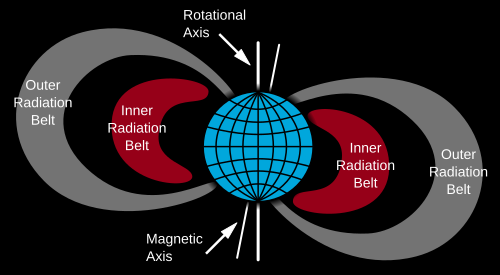
\includegraphics[width=0.95\paperwidth, height=0.80\paperheight, keepaspectratio]{van_allen_belts}}\\
  {\footnotesize Cross-section of Earth's Van Allen radiation belts. Credit: Booyabazooka / NASA, public domain.}
\end{frame}

% ── Aurorae ────────────────────────────────────────────────
\begin{frame}{Aurorae: light from the magnetosphere}
  \begin{columns}[c]
    \column{\recapfigcolnarrow}
    \centering
    \ipsrecapfig{aurora}
    \source{NASA/ISS}

    \column{\recaptextcolwide}
    Solar wind particles channelled along field lines to polar regions:
    \vskip6pt
    \begin{itemize}
      \item \textbf{Green:} excited O at 100--200~km (557.7~nm)
      \item \textbf{Red:} excited O at 200--400~km (630.0~nm)
      \item \textbf{Blue/violet:} excited $\mathrm{N_2}$ bands
    \end{itemize}
    \vskip6pt
    Observed on Jupiter, Saturn, and Uranus: any magnetised planet.
  \end{columns}
\end{frame}

% ── Auroral physics ──────────────────────────────────────
\begin{frame}{Why aurorae happen at the poles, and Jupiter's}
  \begin{itemize}\setlength\itemsep{2pt}
    \item The dipole focuses incoming particles toward the magnetic poles; the polar \textbf{cusps} give the solar wind direct access to the atmosphere
    \item Electrons accelerated by tail reconnection precipitate down the field lines at 1--100 keV and reach 100--400 km altitude; the emission lines are fingerprints of the excited species
    \item \textbf{Jupiter:} $10^{13}$--$10^{14}$ W of UV power, $10^3$--$10^4\times$ Earth's, powered by the $\sim$10 h rotation and $\sim$1 tonne\,s$^{-1}$ of sulfur and oxygen from Io; Io, Europa and Ganymede leave \textbf{auroral footprints}
  \end{itemize}
  \vskip6pt
  \keyresult{Aurorae map the power a magnetosphere dumps into its atmosphere: solar-wind coupling at Earth, rotation and Io's mass loading at Jupiter.}
  \sourcenote{Connerney et al.\ (2022); Mauk et al.\ (2017)}
\end{frame}

% ── Jupiter aurorae ──────────────────────────────────────

% ════════════════════════════════════════════════════════════
\begin{frame}
  \centering
  \makebox[\linewidth][c]{\includegraphics[width=0.95\paperwidth, height=0.80\paperheight, keepaspectratio]{jupiter_uv_aurora}}\\
  {\footnotesize Jupiter's ultraviolet aurora over an optical image, Hubble Space Telescope. Credit: NASA, ESA, J. Nichols (University of Leicester).}
\end{frame}

\sectionimage{aurora}{Aurora australis. Credit: NASA/ISS}
\section{Recent advances \& outlook}
% ════════════════════════════════════════════════════════════

% ── Recent advances ───────────────────────────────────────
\begin{frame}{Juno: Jupiter's asymmetric dynamo}
  \begin{itemize}
    \item Juno (2016--) has measured Jupiter's gravity and magnetic field in unprecedented detail
    \item Surface field dramatically \textbf{non-dipolar}
    \item Northern hemisphere: intense concentrated ``flux lobe''
    \item ``Great Blue Spot'': a patch of reversed polarity near the equator
    \item Magnetic equator offset from the rotational equator
    \item Implies dynamo operates at relatively shallow depths in the stably-stratified dilute core (Lecture~8)
  \end{itemize}
  \vskip4pt
  \sourcenote{Connerney et al.\ (2022), \textit{Journal of Geophysical Research}}
\end{frame}

\begin{frame}
  \centering
  \makebox[\linewidth][c]{\includegraphics[width=0.95\paperwidth, height=0.65\paperheight, keepaspectratio]{jupiter_great_blue_spot}}\\
  {\footnotesize Jupiter's surface radial field after Juno's prime mission (top) and before Juno (bottom): yellow and red mark outward flux, blue inward, and the surface field is strongly non-dipolar. The Great Blue Spot is an intense localised patch of inward flux near the equator, invisible in the low-resolution pre-Juno map. The morphology places the dynamo in a deep but not razor-thin shell of metallic hydrogen. Credit: NASA/JPL-Caltech/SwRI (PIA25040).}
\end{frame}

\begin{frame}{Missions to cores and dynamos}
  \begin{itemize}\setlength\itemsep{3pt}
    \item \textbf{BepiColombo} (ESA/JAXA, launched 2018): flybys 2021--2025 confirmed the weak, active, offset dipole; the two orbiters (MPO, MMO) will map it from polar orbit after the late-2026 orbit insertion
    \item \textbf{JUICE} (launched 2023, Jupiter 2031, Ganymede orbit 2034): separates Ganymede's intrinsic field from the induced ocean signature
    \item \textbf{MAVEN} (2014--): Mars loses $\sim$2--3 kg\,s$^{-1}$, mostly H and photochemically escaping O, faster during solar storms; over 4 Gyr about 0.8 bar of CO$_2$, the link from a dead dynamo to a thin atmosphere (Lecture 5)
    \item \textbf{Psyche} (launched 2023, arrival 2029): a $\sim$220 km M-type asteroid of bulk density $\sim$4 g\,cm$^{-3}$, a candidate exposed planetesimal core; its magnetometer tests for remnant magnetisation
  \end{itemize}
  \vskip4pt
  \sourcenote{Benkhoff et al.\ (2021); Grasset et al.\ (2013); Jakosky et al.\ (2018); Elkins-Tanton et al.\ (2017)}
\end{frame}

\begin{frame}{Open questions in planetary magnetism}
  \begin{itemize}\setlength\itemsep{3pt}
    \item \textbf{When did the inner core nucleate}, and how did Earth sustain a dynamo before it? (most estimates 0.5--1 Gyr ago)
    \item \textbf{Why does Venus have no detectable field?} Inner core, rotation, or tectonics?
    \item \textbf{Why is Mercury's field so weak yet active}, and what drives Ganymede's?
    \item \textbf{How do Uranus and Neptune generate multipolar fields?}
    \item \textbf{Will Earth reverse soon?} No reliable prediction method exists
    \item \textbf{How important are magnetic fields for habitability?}
  \end{itemize}
\end{frame}

% ── Psyche mission ────────────────────────────────────────

% ── Open questions ──────────────────────────────────────

\begin{frame}{Looking ahead to Lecture 5}
  This lecture ended with a planet that has a core, a mantle, a magnetic field, and a freshly outgassed secondary atmosphere.
  \vskip8pt
  \begin{itemize}
    \item Lecture 5 (dr.\ Mara Attia) picks up that atmosphere: primary, secondary, and tertiary atmospheres
    \item Pressure and temperature with height: hydrostatic equilibrium
    \item The greenhouse effect and planetary energy balance
    \item How atmospheres are lost to space; magnetic shielding is one control on escape, but thermal escape proceeds regardless
  \end{itemize}
  \vskip8pt
  \keyresult{Differentiation builds the planet; the atmosphere it outgasses is where climate and habitability are decided.}
\end{frame}

% ── Summary ────────────────────────────────────────────────
\begin{frame}{Summary}
  \begin{enumerate}
    \item Magma oceans drive \textbf{metal--silicate separation}: iron sinks, silicates float
    \item Hf--W chronometry gives a two-stage age of $\sim$30~Myr for Earth's core formation, a lower limit; protracted accretion and partial equilibration place completion within $\sim$100~Myr
    \item Magma ocean crystallisation creates chemically distinct layers (crust, mantle reservoirs)
    \item Dynamos require: conducting fluid + convection + sufficient Rm ($\gtrsim$10--100)
    \item Earth's $\mathrm{Rm} \approx 1750$: vigorous dynamo action
    \item Mars lost its dynamo between $\sim$4.1 and 3.7~Ga (possibly intermittent, Mittelholz 2020) $\rightarrow$ atmospheric erosion
    \item Venus has no detectable field: likely a combination of stagnant-lid tectonics, slow rotation, and/or absence of an inner core
  \end{enumerate}
\end{frame}

% ── Final slide ─────────────────────────────────────────────
\begin{frame}[plain,noframenumbering]
  \begin{tikzpicture}[remember picture, overlay]
    \ipscontain{title_background}
    \fill[ipsPrimary, opacity=0.70] (current page.north west) rectangle (current page.south east);
  \end{tikzpicture}
  \vfill
  \begin{center}
    {\color{white}\Large\bfseries Questions?}
    \vskip20pt
    {\color{white!85}\large Next: Lecture 5, Atmospheres I: composition, structure \& energy balance (Mara Attia)}\\[4pt]
    {\color{white!85}\small Mon 21 Sep, 15:00--17:00, room 5419.0161 (Collegezaal)}\\[12pt]
    {\color{white!85}\small Next tutorial: Fri 25 Sep, 13:00--15:00, room 5419.0161 (Collegezaal)}\\[20pt]
    {\color{white!70}\small \texttt{https://ips.formingworlds.space}}
  \end{center}
  \vfill
\end{frame}

\end{document}
